%%%%%%%%%%%%%%%%%%%%%%%%%%%%%%%%%%%%%%
%This is the article LaTeX template for the RSC journal Faraday Discussions
%Copyright The Royal Society of Chemistry 2010
%%%%%%%%%%%%%%%%%%%%%%%%%%%%%%%%%%%%%%


\documentclass[8.5pt,twoside]{article}
\special{papersize=234mm,156mm}
%\oddsidemargin -1.2cm
%\evensidemargin -1.2cm
%\textwidth 18cm
%\headheight 1.0in
%\topmargin -3.5cm
%\textheight 22cm
\usepackage[super,sort&compress,comma]{natbib} 
%\usepackage{mhchem}
\usepackage{times,mathptm}
\usepackage{sectsty}
\usepackage{balance} 
\usepackage[text={11.3cm,20.4cm},centering]{geometry} 

\usepackage{graphicx} %eps figures can be used instead
\usepackage{lastpage}
\usepackage[format=plain,justification=raggedright,singlelinecheck=false,font=small,labelfont=bf,labelsep=space]{caption} 
\usepackage{fancyhdr}
\pagestyle{fancy}


\begin{document}


\thispagestyle{plain}
\fancypagestyle{plain}{
\fancyhead[L]{
\includegraphics[height=8pt]{headers/LH}}
\fancyhead[C]{\hspace{-1cm}
\includegraphics[height=15pt]{headers/CH}}
\fancyhead[R]{
\includegraphics[height=10pt]{headers/RH}\vspace{-0.2cm}}
\renewcommand{\headrulewidth}{1pt}}
\renewcommand{\thefootnote}{\fnsymbol{footnote}}
\renewcommand\footnoterule{\vspace*{1pt}% 
\hrule width 11.3cm height 0.4pt \vspace*{5pt}} 
\setcounter{secnumdepth}{5}



\makeatletter 
\renewcommand{\fnum@figure}{\textbf{Fig.~\thefigure~~}}
\def\subsubsection{\@startsection{subsubsection}{3}{10pt}{-1.25ex plus -1ex minus -.1ex}{0ex plus 0ex}{\normalsize\bf}} 
\def\paragraph{\@startsection{paragraph}{4}{10pt}{-1.25ex plus -1ex minus -.1ex}{0ex plus 0ex}{\normalsize\textit}} 
\renewcommand\@biblabel[1]{#1}            
\renewcommand\@makefntext[1]% 
{\noindent\makebox[0pt][r]{\@thefnmark\,}#1}
\makeatother 
\sectionfont{\large}
\subsectionfont{\normalsize} 

\fancyfoot{}
\fancyfoot[LO,RE]{\vspace{-7pt}
\includegraphics[height=8pt]{headers/LF}}
\fancyfoot[CO]{\vspace{-7pt}\hspace{5.9cm}
\includegraphics[height=7pt]{headers/RF}}
\fancyfoot[CE]{\vspace{-6.6pt}\hspace{-7.2cm}
\includegraphics[height=7pt]{headers/RF}}
\fancyfoot[RO]{\scriptsize{\sffamily{1--\pageref{LastPage} ~\textbar  \hspace{2pt}\thepage}}}
\fancyfoot[LE]{\scriptsize{\sffamily{\thepage~\textbar\hspace{3.3cm} 1--\pageref{LastPage}}}}
\fancyhead{}
\renewcommand{\headrulewidth}{1pt} 
\renewcommand{\footrulewidth}{1pt}
\setlength{\arrayrulewidth}{1pt}
\setlength{\columnsep}{6.5mm}
\setlength\bibsep{1pt}

\noindent\LARGE{\textbf{This is the title$^\dag$}}
\vspace{0.6cm}

\noindent\large{\textbf{Full Name,$^{\ast}$\textit{$^{a}$} Full Name,\textit{$^{b\ddag}$} and
Full Name\textit{$^{a}$}}}\vspace{0.5cm}
%Please note that \ast indicates the corresponding author(s) but no footnote text is required. 


\noindent\textit{\small{\textbf{Received Xth XXXXXXXXXX 20XX, Accepted Xth XXXXXXXXX 20XX\newline
First published on the web Xth XXXXXXXXXX 200X}}}

\noindent \textbf{\small{DOI: 10.1039/c000000x}}
\vspace{0.6cm}


\noindent \normalsize{The abstract should be a single paragraph which summarises the content of the article. Any references in the abstract should be written out in full \textit{e.g.} [Surname \textit{et al., Journal Title}, 2000, \textbf{35}, 3523].}
\vspace{0.5cm}

\section{This is the section heading style}
%Footnotes
\footnotetext{\dag~Electronic Supplementary Information (ESI) available: [details of any supplementary information available should be included here]. See DOI: 10.1039/c000000x/}

%Please use \dag to cite the ESI in the main text of the article.
%If you article does not have ESI please remove the the \dag symbol from the title and the above footnotetext.

\footnotetext{\textit{$^{a}$~Address, Address, Town, Country. Fax: XX XXXX XXXX; Tel: XX XXXX XXXX; E-mail: xxxx@aaa.bbb.ccc}}
\footnotetext{\textit{$^{b}$~Address, Address, Town, Country. }}

%additional addresses can be cited as above using the lower-case letters, c, d, e... If all authors are from the same address, no letter is required

\footnotetext{\ddag~Additional footnotes to the title and authors can be included \emph{e.g.}\ `Present address:' or `These authors contributed equally to this work' as above using the symbols: \ddag, \textsection, and \P. Please place the appropriate symbol next to the author's name and include a \texttt{\textbackslash footnotetext} entry in the the correct place in the list.}


The main text of the article\cite{Mena2000} should appear here.

\subsection{This is the subsection heading style}
Section headings can be typeset with and without numbers.\cite{Abernethy2003}

\subsubsection{This is the subsubsection style.~~} These headings should end in a full point.  

\paragraph{This is the next level heading.~~} For this level please use \texttt{\textbackslash paragraph}. These headings should also end in a full point.

\section{Equations}

Equations can be typeset inline \textit{e.g.} $ y = mx + c$ or displayed with and without numbers:

 \[ A = \pi r^2 \]

\begin{equation}
  \frac{\mathrm{\gamma}}{\mathrm{\epsilon}x} r^2 = 2r
\end{equation}

\section{Graphics and tables}
\subsection{Graphics}
Graphics should be inserted on the page where they are first mentioned (unless they are equations, which appear in the flow of the text).\cite{Cotton1999}

\begin{figure}[h]
\centering
  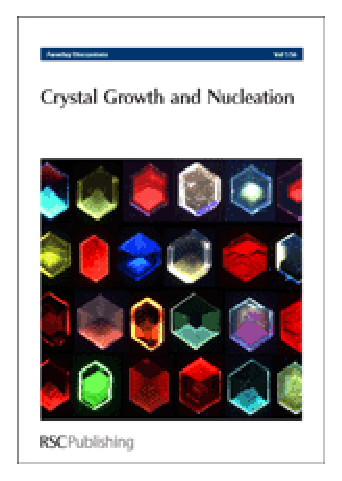
\includegraphics[height=3cm]{example}
  \caption{An example figure caption}
  \label{fgr:example}
\end{figure}

\subsection{Tables}
Tables typeset in RSC house style do not include vertical lines. Table footnote symbols are lower-case italic letters and are typeset at the bottom of the table. Table captions do not end in a full point.\cite{Arduengo1992,Eisenstein2005}


\begin{table}[h]
\small
\centering
  \caption{~An example of a caption to accompany a table}
  \label{tbl:example}
  \begin{tabular}{l l l l} %table columns can also be centre- or right-aligned using 'c' or 'r' instead of 'l' here
    \hline
    Header one/units & Header two & Header three \\
    \hline
    1 & 2 & 3 \\
    4 & 5 & 6 \\
    7 & 8 & 9 \\
    10 & 11 & 12 \\
    \hline
  \end{tabular}
\end{table}


Adding notes to tables can be complicated.  Perhaps the easiest
method is to generate these manually.

You can also put lists into the text. You can have bulleted or numbered lists of almost any kind. 
The \texttt{mhchem} package can also be used so
that formulae are easy to input: 
%\texttt{\textbackslash ce\{H2SO4\}} gives \ce{H2SO4}. 



The conclusions section should come at the end of article. For the reference section, the style file rsc.bst can be used to generate the correct reference style.\footnote[4]{Footnotes should appear here. These might include comments relevant to but not central to the matter under discussion, limited experimental and spectral data, and crystallographic data.}
 %For footnotes in the main text of the article please number the footnotes to avoid duplicate symbols. e.g.  \footnote[num]{your text} the corresponding author \ast counts as footnote 1, ESI as footnote 2, e.g. if there is no ESI, please start at [num]=[2], if ESI is cited in the title please start at [num]=[3] etc. 

\section*{Acknowledgements}
Acknowledgements can be included here. This section does not normally have a section number.


%The \balance command can be used to balance the columns on the final page if desired. It should be placed anywhere within the first column of the last page.

%\balance

%If notes are included in your references you can change the title using the following command.
%\renewcommand\refname{Notes and references}

\footnotesize{
\bibliography{rsc} %your .bib file
\bibliographystyle{rsc}
}

\end{document}
